\chapter{Résultats et perspectives}

\section{Résultats}
\begin{itemize}
  \item surface
\end{itemize}

Nous sommes donc capables, étant donné un complexe stocké dans un fichier \textit{.pdb},
d'afficher ce complexe et de visualiser la surface de de contact dans Meshlab
(voir figure \ref{fig::affichage_final}).

\begin{figure}[ht]
\centering
\begin{subfigure}{0.45\textwidth}
  \centering
  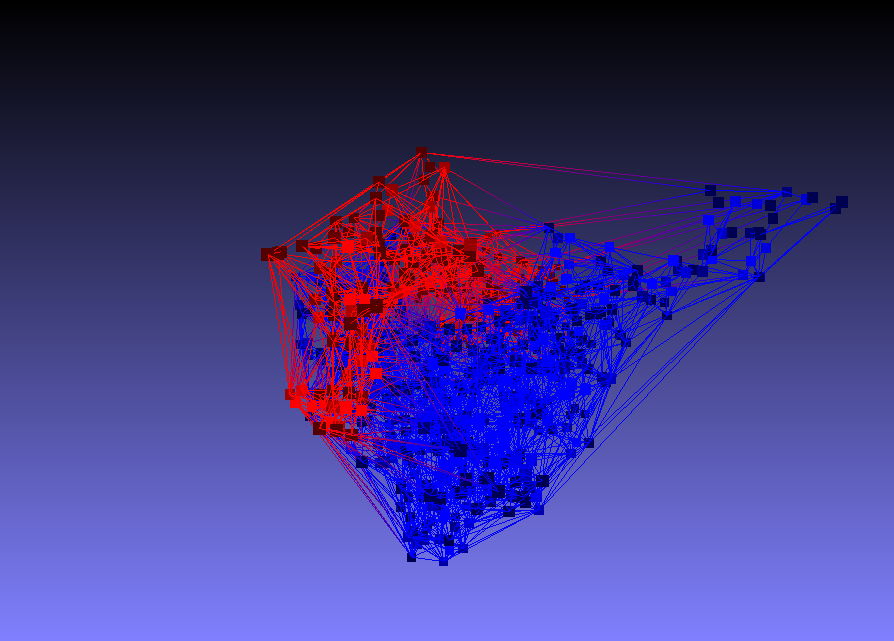
\includegraphics[width=\textwidth]{figures/final_no_surf.png}
  \caption{Complexe}
  \label{fig::complexe}
\end{subfigure}%
\begin{subfigure}{0.1\textwidth}
  \centering
  $\Longrightarrow$
\end{subfigure}%
\begin{subfigure}{0.45\textwidth}
  \centering
  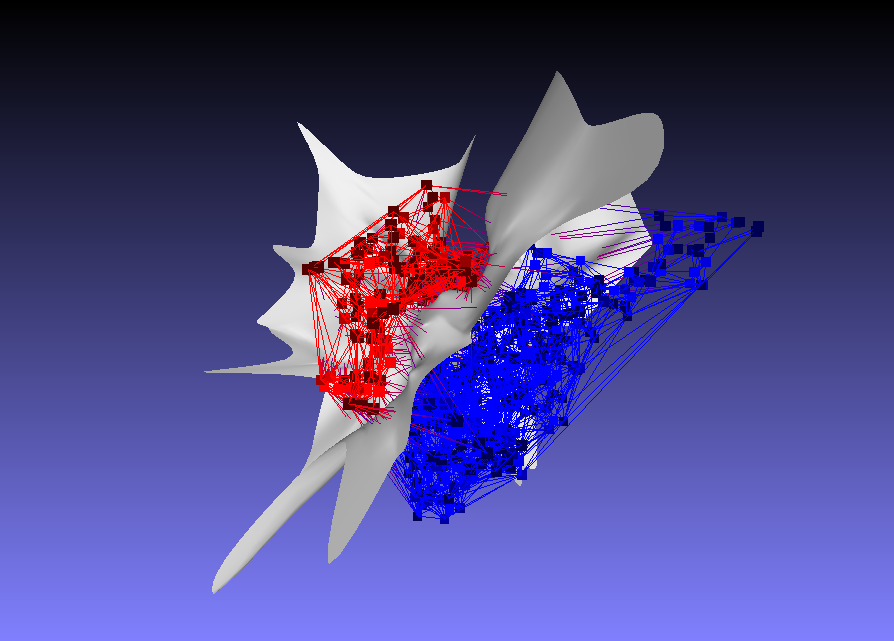
\includegraphics[width=\textwidth]{figures/final_with_surf.png}
  \caption{Interface de contact}
  \label{fig::interface}
\end{subfigure}
\caption{Affichage de l'interface entre deux protéines}
\label{fig::affichage_final}
\end{figure}
\section{Limitations et problèmes rencontrés}
\begin{itemize}
  \item Compilation
  \item CGAL, structures
\end{itemize}

\section{Perspectives}
\begin{itemize}
  \item Fonctionnalités
\end{itemize}
